% Use only LaTeX2e, calling the article.cls class and 12-point type.

\documentclass[11pt]{article}
\usepackage[round,semicolon]{natbib}
\usepackage[margin=1.25in]{geometry}
\usepackage{kpfonts}

\usepackage{seqsplit}
\usepackage{placeins}

\usepackage{newfloat}
\usepackage[labelfont=bf]{caption}
\usepackage{nameref}
\usepackage{rotating}
\usepackage{color}
\usepackage{float}

\setcounter{topnumber}{8}
\setcounter{bottomnumber}{8}
\setcounter{totalnumber}{8}
\renewcommand{\topfraction}{1}
\renewcommand{\bottomfraction}{1}
\renewcommand{\textfraction}{0}
\renewcommand{\floatpagefraction}{1}

\usepackage[font=small,labelfont=bf]{caption}

\usepackage{newfloat}
\DeclareFloatingEnvironment[name={Figure}]{suppfigure}
\renewcommand{\thesuppfigure}{S\arabic{suppfigure}}
\DeclareFloatingEnvironment[name={Table}]{supptable}
\renewcommand{\thesupptable}{S\arabic{supptable}}
\DeclareFloatingEnvironment[name={File}]{suppfile}
\renewcommand{\thesuppfile}{S\arabic{suppfile}}

\definecolor{darkblue}{rgb}{0, 0.0, 0.6}

\usepackage{hyperref}
\hypersetup{colorlinks,citecolor=blue,linkcolor=blue,urlcolor=blue}

\usepackage{seqsplit}

\usepackage{array}
\newcolumntype{R}[1]{>{\raggedright\arraybackslash}p{#1}}
\newcolumntype{C}[1]{>{\centering\let\newline\\\arraybackslash\hspace{0pt}}m{#1}}

\newcommand{\comment}[1]{{\color{red}[\textsl{#1}]}}

\usepackage{setspace}

\renewcommand{\topfraction}{1}
\renewcommand{\bottomfraction}{1}
\renewcommand{\textfraction}{0}
\renewcommand{\floatpagefraction}{1}


\title{Deep mutational scanning of an H3 hemagglutinin can inform evolutionary forecasting of human H3N2 influenza virus} 

\author{
Juhye M. Lee$^{1,4,5,\dagger}$ \and 
John Huddleston$^{2,6,\dagger}$ \and 
Michael B. Doud$^{1,4,5}$ \and 
Kathryn A. Hooper$^{1,6}$ \and
Trevor Bedford$^{2,3*}$ and \and 
Jesse D. Bloom$^{1,3,4*}$
\\
\scriptsize{$^1$Basic Sciences Division, $^2$Vaccine and Infectious Diseases Division, and $^3$Computational Biology Program,} \\
\scriptsize{Fred Hutchinson Cancer Research Center, Seattle, WA, USA} \\
\scriptsize{$^4$Department of Genome Sciences, $^5$Medical Scientist Training Program, and $^6$Molecular and Cellular Biology Program,} \\
\scriptsize{University of Washington, Seattle, WA, USA} \\
\scriptsize{$^{\dagger}$These authors contributed equally} \\
\scriptsize{$^*$Correspondence: \href{trevor@bedford.io}{trevor@bedford.io}, \href{jbloom@fredhutch.org}{jbloom@fredhutch.org}}
}

\date{}


\begin{document}

\maketitle
\onehalfspacing

\begin{abstract}
Abstract text.
\end{abstract}

\section*{INTRODUCTION}
Very rough outline:
\begin{itemize}
\item Mutations are rampant in the evolution of human influenza virus. Seasonal H3N2 influenza virus in particular rapidly accumulates mutations.
\item The evolution of H3N2 is also characterized by clade competition and population turnover.
\item There have been efforts to predict evolutionary success.
\item Mutations that contribute to antigenic evolution largely determine strain success.
\item RNA viruses can accumulate deleterious mutations, and because the influenza does not appreciably recombine, deleterious mutations are linked to beneficial ones.
\item Mutations in HA that impact viral growth may influence strain success.
\item We need to understand the functional impact of mutations in HA.
\item Previously, we measured the effect of all possible single amino-acid mutations to an H1 hemagglutinin from the A/WSN/1933 (H1N1) strain~\citep{thyagarajan2014inherent,doud2016accurate}. 
\item However, this is a highly lab-adapted strain, and the measurements in this strain may not be particularly relevant for studying mutational processes of more contemporaneous strains circulating in the human population.
\item We chose to study the Perth/2009 H3 HA.
\item This also enabled a comparison of how the preferences have shifted for two diverged HA's.
\end{itemize}

\section*{RESULTS}
\label{sec:results}

\subsection*{Deep mutational scanning of HA from a recent strain of human H3N2 influenza virus}
We performed a deep mutational scan of H3 HA from the A/Perth/16/2009 (H3N2) strain. 
This strain was the H3N2 component of the influenza vaccine from 2010-2012.
The HA gene we used in our experiments carries two mutations, G78D and T212I, relative to the Perth/2009 HA sequence deposited in GenBank.
The G78D mutation has appeared sporadically at low frequency in natural H3N2 sequences. 
Although the T212I mutation is not appreciable in nature \comment{reword}, the T212A mutation rose to fixation in the human population in $\sim$2011.
We found that the G78D-T212I Perth/2009 HA mutant supported viral growth to $\sim$15- to 20-fold higher titers than the wildtype HA.
%We first generated virus carrying the wildtype Perth/2009 HA and NA and the WSN internal genes by reverse genetics, and serially passaged the virus in cell culture a total of six times.
%This passaging was completed to allow the virus to adapt to growth in cell culture and to find cell-culture adaptation mutations that emerged during the course of passaging.
%Two mutations, G78D and T212I, arose together from passaging.
We therefore decided to perform all deep mutational scanning experiments in the background of the Perth/2009 HA carrying these two mutations to support higher viral growth.

We mutagenized the HA gene to create mutant plasmid libraries encompassing all 567 codons and harboring an average of $\sim$1.4 codon mutations per clone.
We then generated mutant virus libraries from the mutant plasmids using a helper virus system that enables the efficient generation of complex virus libraries~\citep{doud2016accurate} (Figure~\ref{fig:dms_overview}A).
In order to reduce biosafety concerns and to maximize viral titers, we used an HA-deficient helper virus carrying WSN/1933 internal and NA genes to rescue the mutant viruses.
Additionally, we used MDCK-SIAT1 cells constitutively expressing the TMPRSS2 protease, which facilitates HA cleavage and activation in the human airway \comment{cite B\"{o}ttcher 2006 JVI, B\"{o}ttcher-Friebertsh\"{a}user 2010 JVI}.
All of the experiments were completed in full biological triplicate (Figure~\ref{fig:dms_overview}B). 
We also passaged and deep sequenced library 3 in technical replicate (denoted as library 3-1 and 3-2) to gauge to the amount of experimental noise occurring \textit{within} a single biological replicate.

Figure~\ref{fig:dms_overview}C shows the mutation frequencies of the mutant plasmids, mutant viruses, wildtype plasmids and wildtype viruses determined from deep sequencing. 
There is selection against non-functional HA variants as revealed by the reduced mutation frequencies of the mutant viruses compared to their starting frequencies in the mutant plasmids.
Specifically, stop codons were purged to 20-45\% of their original starting frequencies, after correcting for error rates from the wildtype controls.
Although the majority of stop codons were purged, incomplete purging of stop codons is likely due to complementation of defective viral particles by infectious virions. 
We also observed purging of most nonsynonymous mutations to 30-40\% of their initial starting frequencies after error correction, suggesting strong selection against deleterious HA variants.

We next quantified the reproducibility of our deep mutational scanning measurements across biological and technical replicates. 
We inferred the amino-acid preferences at each site in the Perth/2009 HA using the method described in~\cite{bloom2015software} and implemented in the \texttt{dms\_tools2} software [\url{https://jbloomlab.github.io/dms_tools2/}].
These preferences represent an estimate of the 567 sites $\times$ 20 amino acids $=$ 11340 experimental measurements and are normalized to sum to one at each site.
The correlations of the amino-acid preferences between each pair of replicates is shown in Figure~\ref{fig:dms_overview}D.
The biological replicates are fairly well-correlated, with a Pearson's $R$ ranging from 0.69 to 0.78. 
Replicate 1 exhibits the least amount of correlation with the other biological replicates, consistent with the observation that this replicate showed the weakest selection against stop and nonsynonymous mutations and might therefore be subject to more experimental noise.
Of note, the two technical replicates 3-1 and 3-2 were only slightly more reproducible than that between biological replicates.
This suggests that bottlenecking of the virus library during the low MOI passage contributes to much of the noise observed in our experiments, as we are only able to passage a finite number of viral particles.

\begin{figure}
\centerline{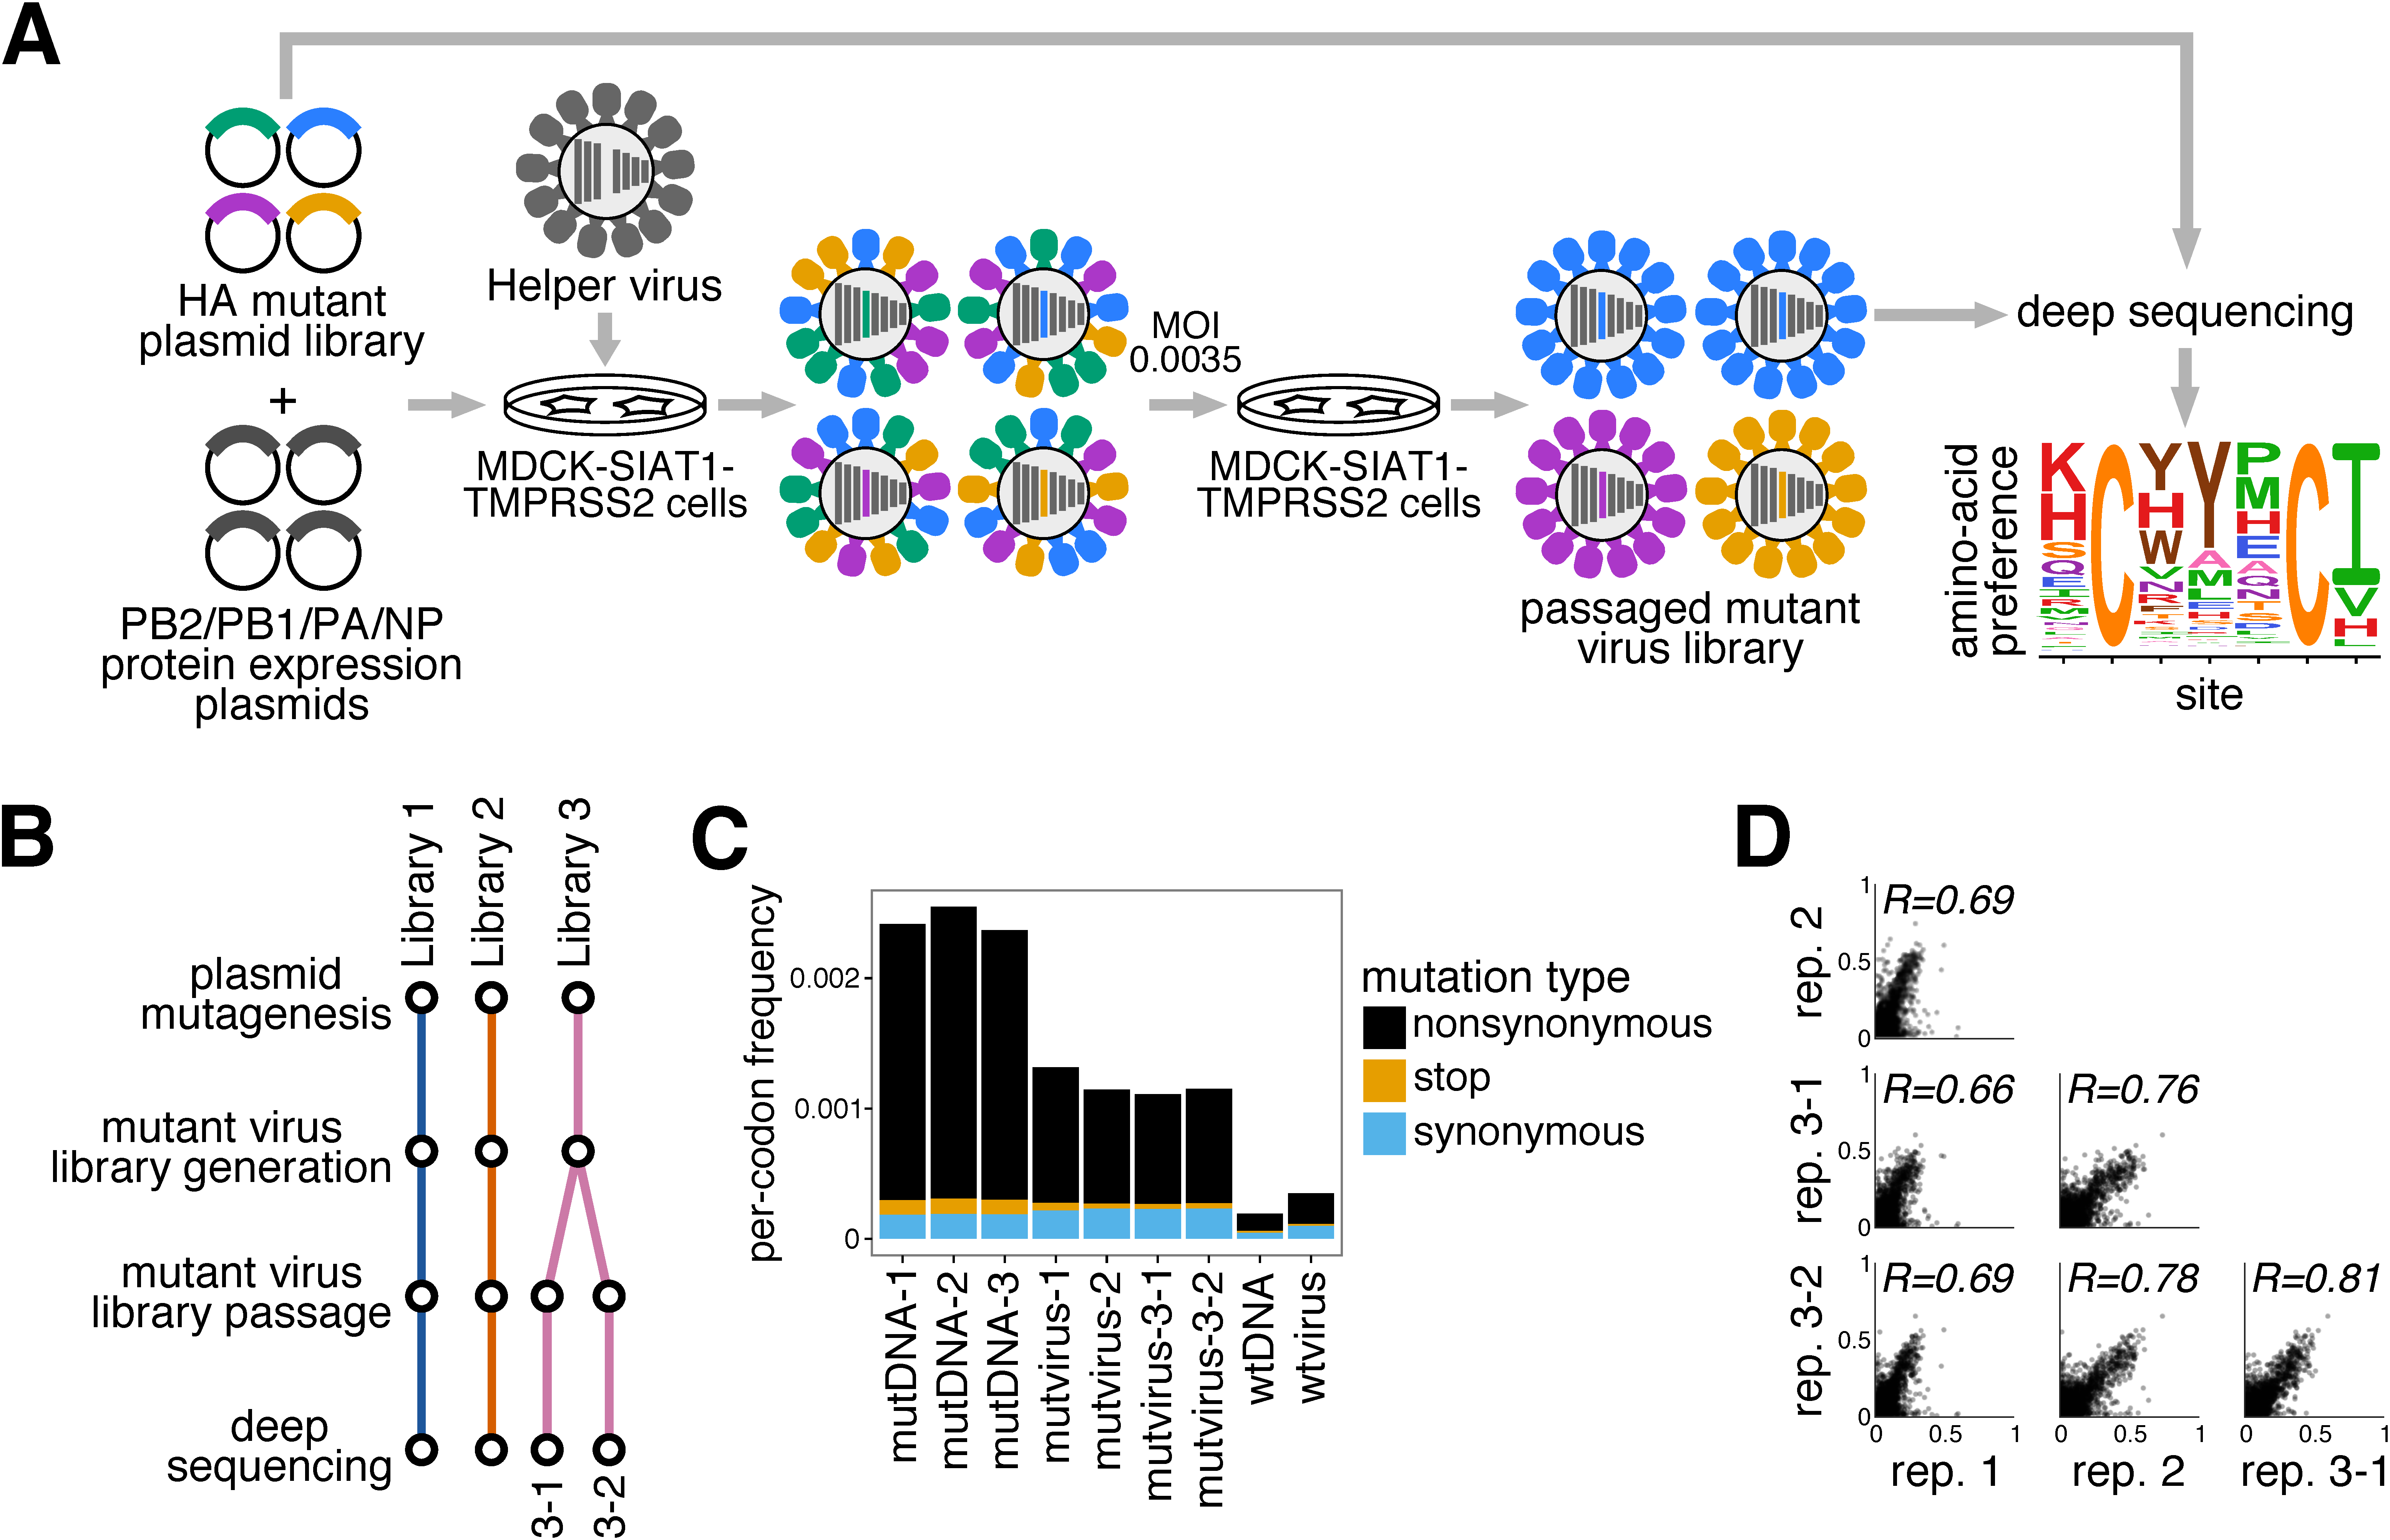
\includegraphics[width=\textwidth]{figs/dms_overview/dms_overview.pdf}}
\caption{\label{fig:dms_overview}
{\bf Deep mutational scanning experiments of H3 HA.}
(A) We used a helper virus approach previously described in Doud (2016) to generate the mutant virus libraries. 
We transfected MDCK-SIAT1-TMPRSS2 cells with the mutant plasmid library carrying all possible amino-acid mutations to the A/Perth/16/2009 (H3N2) HA, in addition to protein expression plasmids encoding the viral ribonucleoprotein complex. 
After transfection, we infected the cells with an HA-deficient helper virus carrying all of the WSN/1933 (H1N1) influenza genes. 
We then passaged the initially generated pool of mutant viruses at low MOI to establish a genotype-phenotype linkage and select for functional HA variants. 
(B) All of the experiments were completed in biological triplicate, starting from independent preps of the wildtype HA genes to create the mutant plasmids. 
In addition, we passaged and deep sequenced library 3 in technical replicate, denoted 3-1 and 3-2, to estimate the amount of experimental noise within a single biological replicate.
(C) Mutation frequencies of nonsynonymous, stop, and synonymous mutations for the mutant DNA, mutant virus, wildtype DNA, and wildtype virus samples. 
There is selection against nonsynonymous and stop codons in the mutant viruses. 
The percentages signify the frequency of stop codons remaining in the passaged mutant viruses relative to their starting frequency in the mutant plasmid libraries after correcting for the stop codon frequencies in the wildtype DNA and viruses.
(D) The correlations and the Pearson correlation coefficient for the amino-acid preferences between each pair of replicates are shown. 
The biological replicates are fairly well-correlated, as are the technical replicates, indicating some degree of bottlenecking of variants during the viral passage which can contribute to experimental noise. 
}
\end{figure}


\subsection*{The HA preferences improve phylogenetic fit of natural H3 sequences}
How well do the Perth/2009 HA preferences inferred from experimental measurements describe the evolution of H3N2 influenza virus in nature?
This question can be addressed by evaluating how well experimentally informed codon substitution models (ExpCM's) constructed from our laboratory measurements improve phylogenetic fit of H3N2 evolution~\citep{hilton2017phydms}.
The results in Table~\ref{tab:phydms} show that the ExpCM outperforms conventional substitution models in describing the evolution of human H3N2 HA. 
The ExpCM also optimizes a stringency parameter ($\beta$) for the preferences to more closely reflect the strength of selection in nature.
The stringency parameter in the ExpCM is equal to 2.44, which indicates that although the same amino acids are preferred, the strength of selection is more stringent in nature than in our experiments.
Figure~\ref{fig:logoplot} shows a logo plot of the Perth/2009 HA amino-acid preferences rescaled by this stringency parameter.

\begin{table}
\centering
\begin{tabular}{cccc}
\hline
\bf{Model} & \bf{$\Delta$AIC} & \bf{Log Likelihood} & \bf{Stringency} \\ \hline
ExpCM & 0.0 & -8439.33 & $\beta = 2.44, \omega = 0.91$ \\
Goldman-Yang M5 & 2166.06 & -9516.36 & $\omega_{\alpha} = 0.30, \omega_{\beta} = 0.84, \kappa = 5.10$ \\
ExpCM, averaged across sites & 2504.18 & -9691.42 & $\beta = 0.68, \kappa = 5.58, \omega = 0.32$ \\
Goldman-Yang M0 & 2607.92 & -9738.29 & $\kappa = 5.05, \omega = 0.31$ \\
\hline
\end{tabular}
\caption{\label{tab:phydms}
{\bf The site-specific amino-acid preferences are informative for describing human H3N2 evolution in nature.}
We implemented several codon substitution models for phylogenetic fitting of an alignment of human H3N2 HA sequences. 
The maximum likelihood values for each model were compared using the Akaike information criteria ($\Delta$AIC)~\citep{posada2004model}.
An experimentally-informed codon substitution model (ExpCM) built from the preferences averaged across all replicates performs better than conventional substitution models, specifically the M0 and M5 models in~\cite{yang2000codon}.
A non-site-specific ExpCM informed by preferences averaged across all sites does not perform as well as the M5 model, but still has a higher log likelihood than M0.
The optimized parameters for each model are also shown.
}
\end{table}

A closer examination of the logo plot reveals that the preferences generally agree with existing knowledge about HA's biochemistry.
For instance, sites that form structurally important disulfide bridges (sites 52 \& 277, 64 \& 76, 97 \& 139, 281 \& 305, 14 \& 137-HA2, 144-HA2 \& 148-HA2)~\citep{waterfield1981disulphide} possess high preference for cysteine.
At residues involved in receptor binding, there are strong preferences for the amino acids at sites Y98, D190, W153, and S228.
A positively charged amino acid at site 329 is important for cleavage activation of the HA0 precursor, and indeed this site exhibits a high preference for arginine~\citep{kido1992isolation, stech2005new}.
However, a notable exception occurs at the start codon at position -16, which does not show a strong preference for methionine. 
This codon is part of the signal peptide and is cleaved from the mature HA protein.
One possible explanation for why we do not see a strong preference for Met at this site is due to alternative translation initiation occurring at a downstream or upstream start site, as has been described in \comment{need to list citations here, inc. Girard 2011 Infection Genetics and Evolution, Chen 2001 Nat Med}.
% No upstream or downstream "ATG"'s are present. I did find an in-frame "ATC" one codon upstream of the canonical start site (in the non-coding region), and interestingly, all Perth/2009 HA sequences deposited in GenBank have an "ATT" in this non-coding position, including Seema's Perth HA.
% I6M(HA2) mutant slightly increases the fusion pH (Daniels 1985 Cell)
% We see high preference for T,S,Q over the wildtype Ile at site 226. Although Q226 in an H3 background is characterized as having preference for avian-type receptors, most of these studies were done in older H3 strains such as Aichi. Wu 2017 Cell Host Microbe has shown extensive epistasis in the RBS, specifically in the 220-loop, so perhaps the amino acids tolerated in this loop have shifted over time. Indeed the wildtype amino acids at 225 and 226 are different in Perth compared to HK68 and Aichi.

\begin{figure}
\centerline{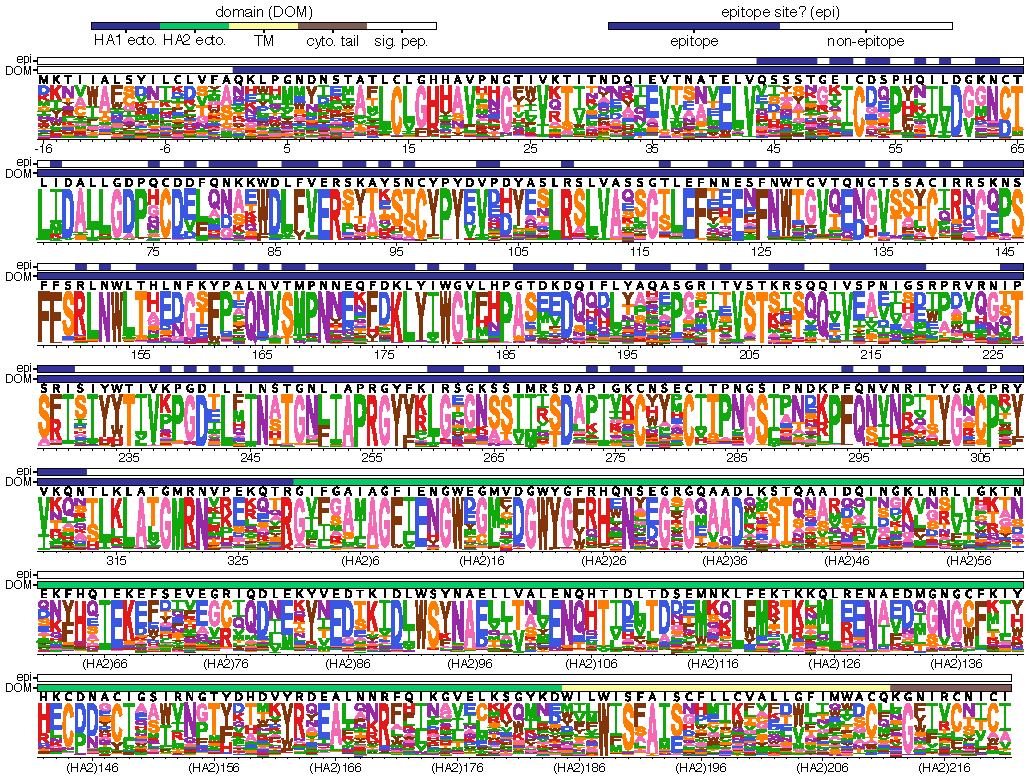
\includegraphics[width=\textwidth]{figs/prefslogoplot/rescaled-avgprefs_prefs.pdf}}
\caption{\label{fig:logoplot}
{\bf The site-specific amino-acid preferences of the Perth/2009 HA.}
This logoplot shows the site-specific amino-acid preferences for the averaged replicates rescaled by the stringency parameter (Table 1) estimated by phydms.
The height of each letter is proportional to its preference at that site, and the preferences for all sites are normalized to sum to 1.
The sites are in H3 numbering.
The top overlay bar shows the relative solvent accessibility.
The bottom overlay bar is colored by the HA domain (sig. pep. = signal peptide, HA1 ecto. = HA1 ectodomain, HA2 ecto. = HA2 ectodomain, TM = transmembrane domain, cyto. tail. = cytoplasmic tail).
The letters directly above each logo indicate the wildtype amino acid at that site.
}
\end{figure}

\subsection*{The H3 stalk is relatively mutationally tolerant}
We next sought to investigate the inherent mutational tolerance of the Perth/2009 HA. 
Figure~\ref{fig:mut_tolerance} shows the mutational tolerance as calculated from the rescaled Perth/2009 H3 preferences and the rescaled WSN/1933 H1 preferences mapped onto the HA crystal structures.
Interestingly, the Perth/2009 H3 stalk is relatively mutationally tolerant compared to the tolerance of the globular head domain. 
In particular, the shorter $\alpha$-helix (helix A) of the stalk domain, antigenic site C, and the most distal portion of the globular head near antigenic site B are all highly mutationally tolerant.
% may add more details here
On the other hand, the head domain of the WSN/1933 H1 is more mutationally tolerant relative to its stalk domain.
The receptor binding pockets of both HA's are relatively mutationally intolerant, although the residues surrounding the receptor binding pocket are fairly tolerant of mutations.
These findings are consistent with the high functional constraint of the receptor binding pocket, while the mutability of sites surrounding the pocket that are under strong immune pressure may contribute to antigenic evolution~\citep{wilson1981structure, wiley1981structural}.

\begin{figure}
\centerline{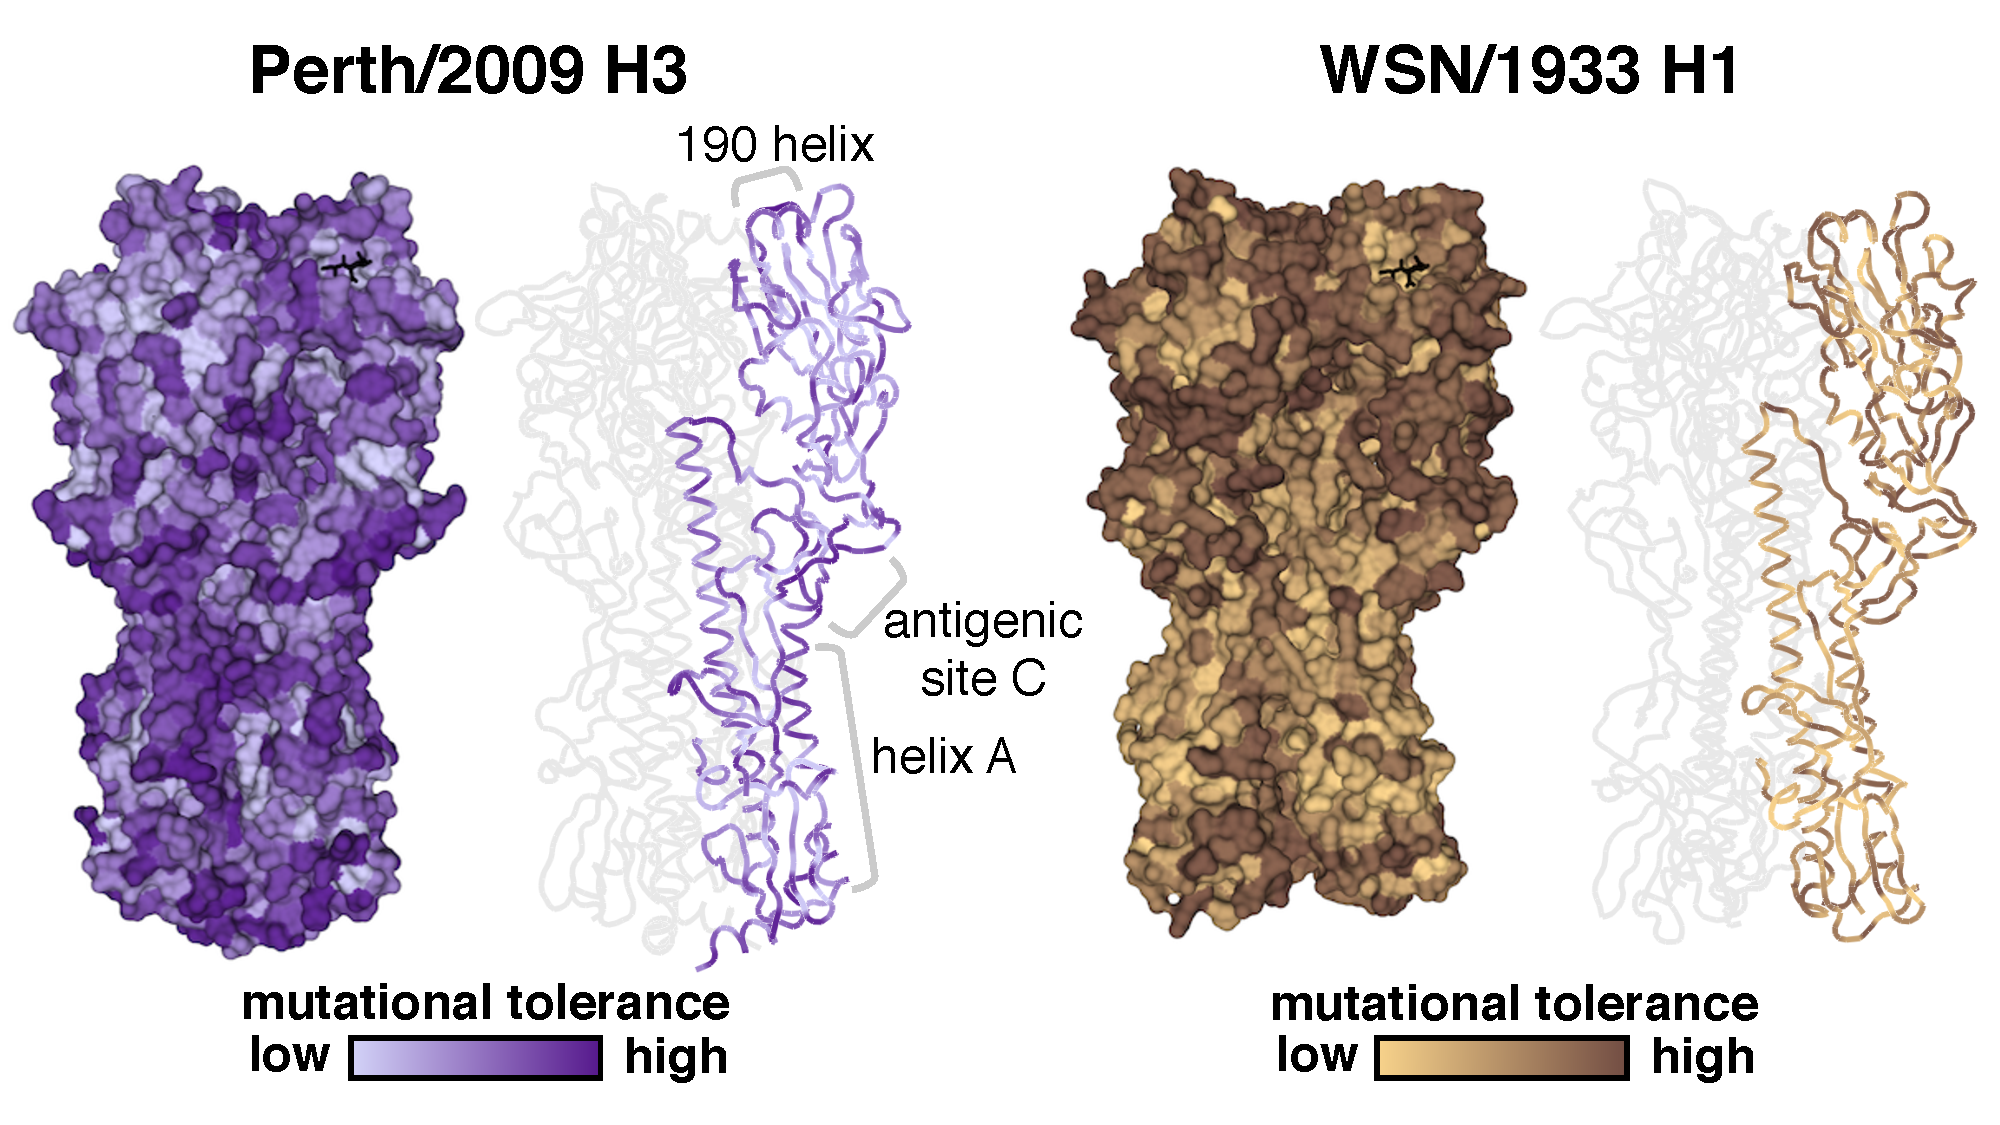
\includegraphics[width=\textwidth]{figs/mut_tolerance/entropy_heatmap.pdf}}
\caption{\label{fig:mut_tolerance}
{\bf Mutational tolerance mapped onto each site of HA.}
Mutational tolerance as calculated by the Shannon entropy of a given site's amino-acid preferences are mapped onto the structure of the H3 trimer (PDB 4O5N;~\cite{lee2014receptor}) and the H1 trimer (PDB 1RVX;~\cite{gamblin2004structure}), with both trimers in approximately the same orientation. 
The site entropies were calculated from the preferences measured in the Perth/2009 H3 (left panel) from this study, or the preferences measured in the WSN/1933 H1 (right panel) from~\cite{doud2016accurate}. 
Lighter shades of blue or red signify low mutational tolerance, while darker shades of blue or red signify high mutational tolerance. 
For each HA, the structure on the left side colors the full HA trimer, while the structure on the right side colors only one of the monomers.
The sialic acid receptor is shown as black sticks.
The Perth/2009 H3 shows relatively high mutational tolerance in the stalk region compared to the head region. 
The head region of the WSN/1933 H1 is mutationally tolerant compared to the relatively intolerant stalk region. 
}
\end{figure}

\subsection*{The H3 preferences reveal differences in seasonal influenza virus lineages}
% The human H3N2 phylogeny has a characteristic ladder-like structure, with a persistent trunk lineage and side branches that rapidly die out.
Do the preferences reveal inherent differences between lineages of human H3N2 influenza virus that have succeeded and those that have died out?
To examine this, we calculated the effect of trunk and side branch mutations from an H3N2 phylogeny, shown in Figure~\ref{fig:trunkvssidebranch}A, from 1968-2012 using our preference dataset. 
Strains with mutations that we measured to be more beneficial to viral growth tend to succeed in nature.
Figure~\ref{fig:trunkvssidebranch}B shows the median log$_{2}$ mutational effects and the interquartile ranges for trunk and side branch mutations in five-year windows for every year from 1968-2012. 
On average, trunk mutations tend to be towards more preferred amino acids compared to side branch mutations, and this was true for all windows.
Next we calculated the effect of all trunk and side branch mutations from the entirety of the phylogenetic tree.
We found that on average, trunk mutations are significantly more favorable than side branch mutations (Figure~\ref{fig:trunkvssidebranch}C).
Because a number of tip nodes are likely from egg- or cell-passaged isolates and our experiments were performed in cell culture, we were curious to see if our measurements would lead to higher estimations of mutational effects for terminal nodes.
We found that terminal node mutations are on average towards less preferred amino acids than internal node mutations, and that both internal and terminal node mutations are significantly less favorable than those on the trunk.
Therefore, strains that have accumulated mutations that we measured in our experiments to be unpreferred generally die out in nature, while more favored mutations  provide a selective advantage to the surviving trunk.
\comment{The average effect of trunk mutations near zero may also suggest that there is a balance between preferred and unpreferred mutations on the trunk.}
These findings demonstrate the importance of the functional impacts of HA mutations in determining lineage success.

\begin{figure}
\centerline{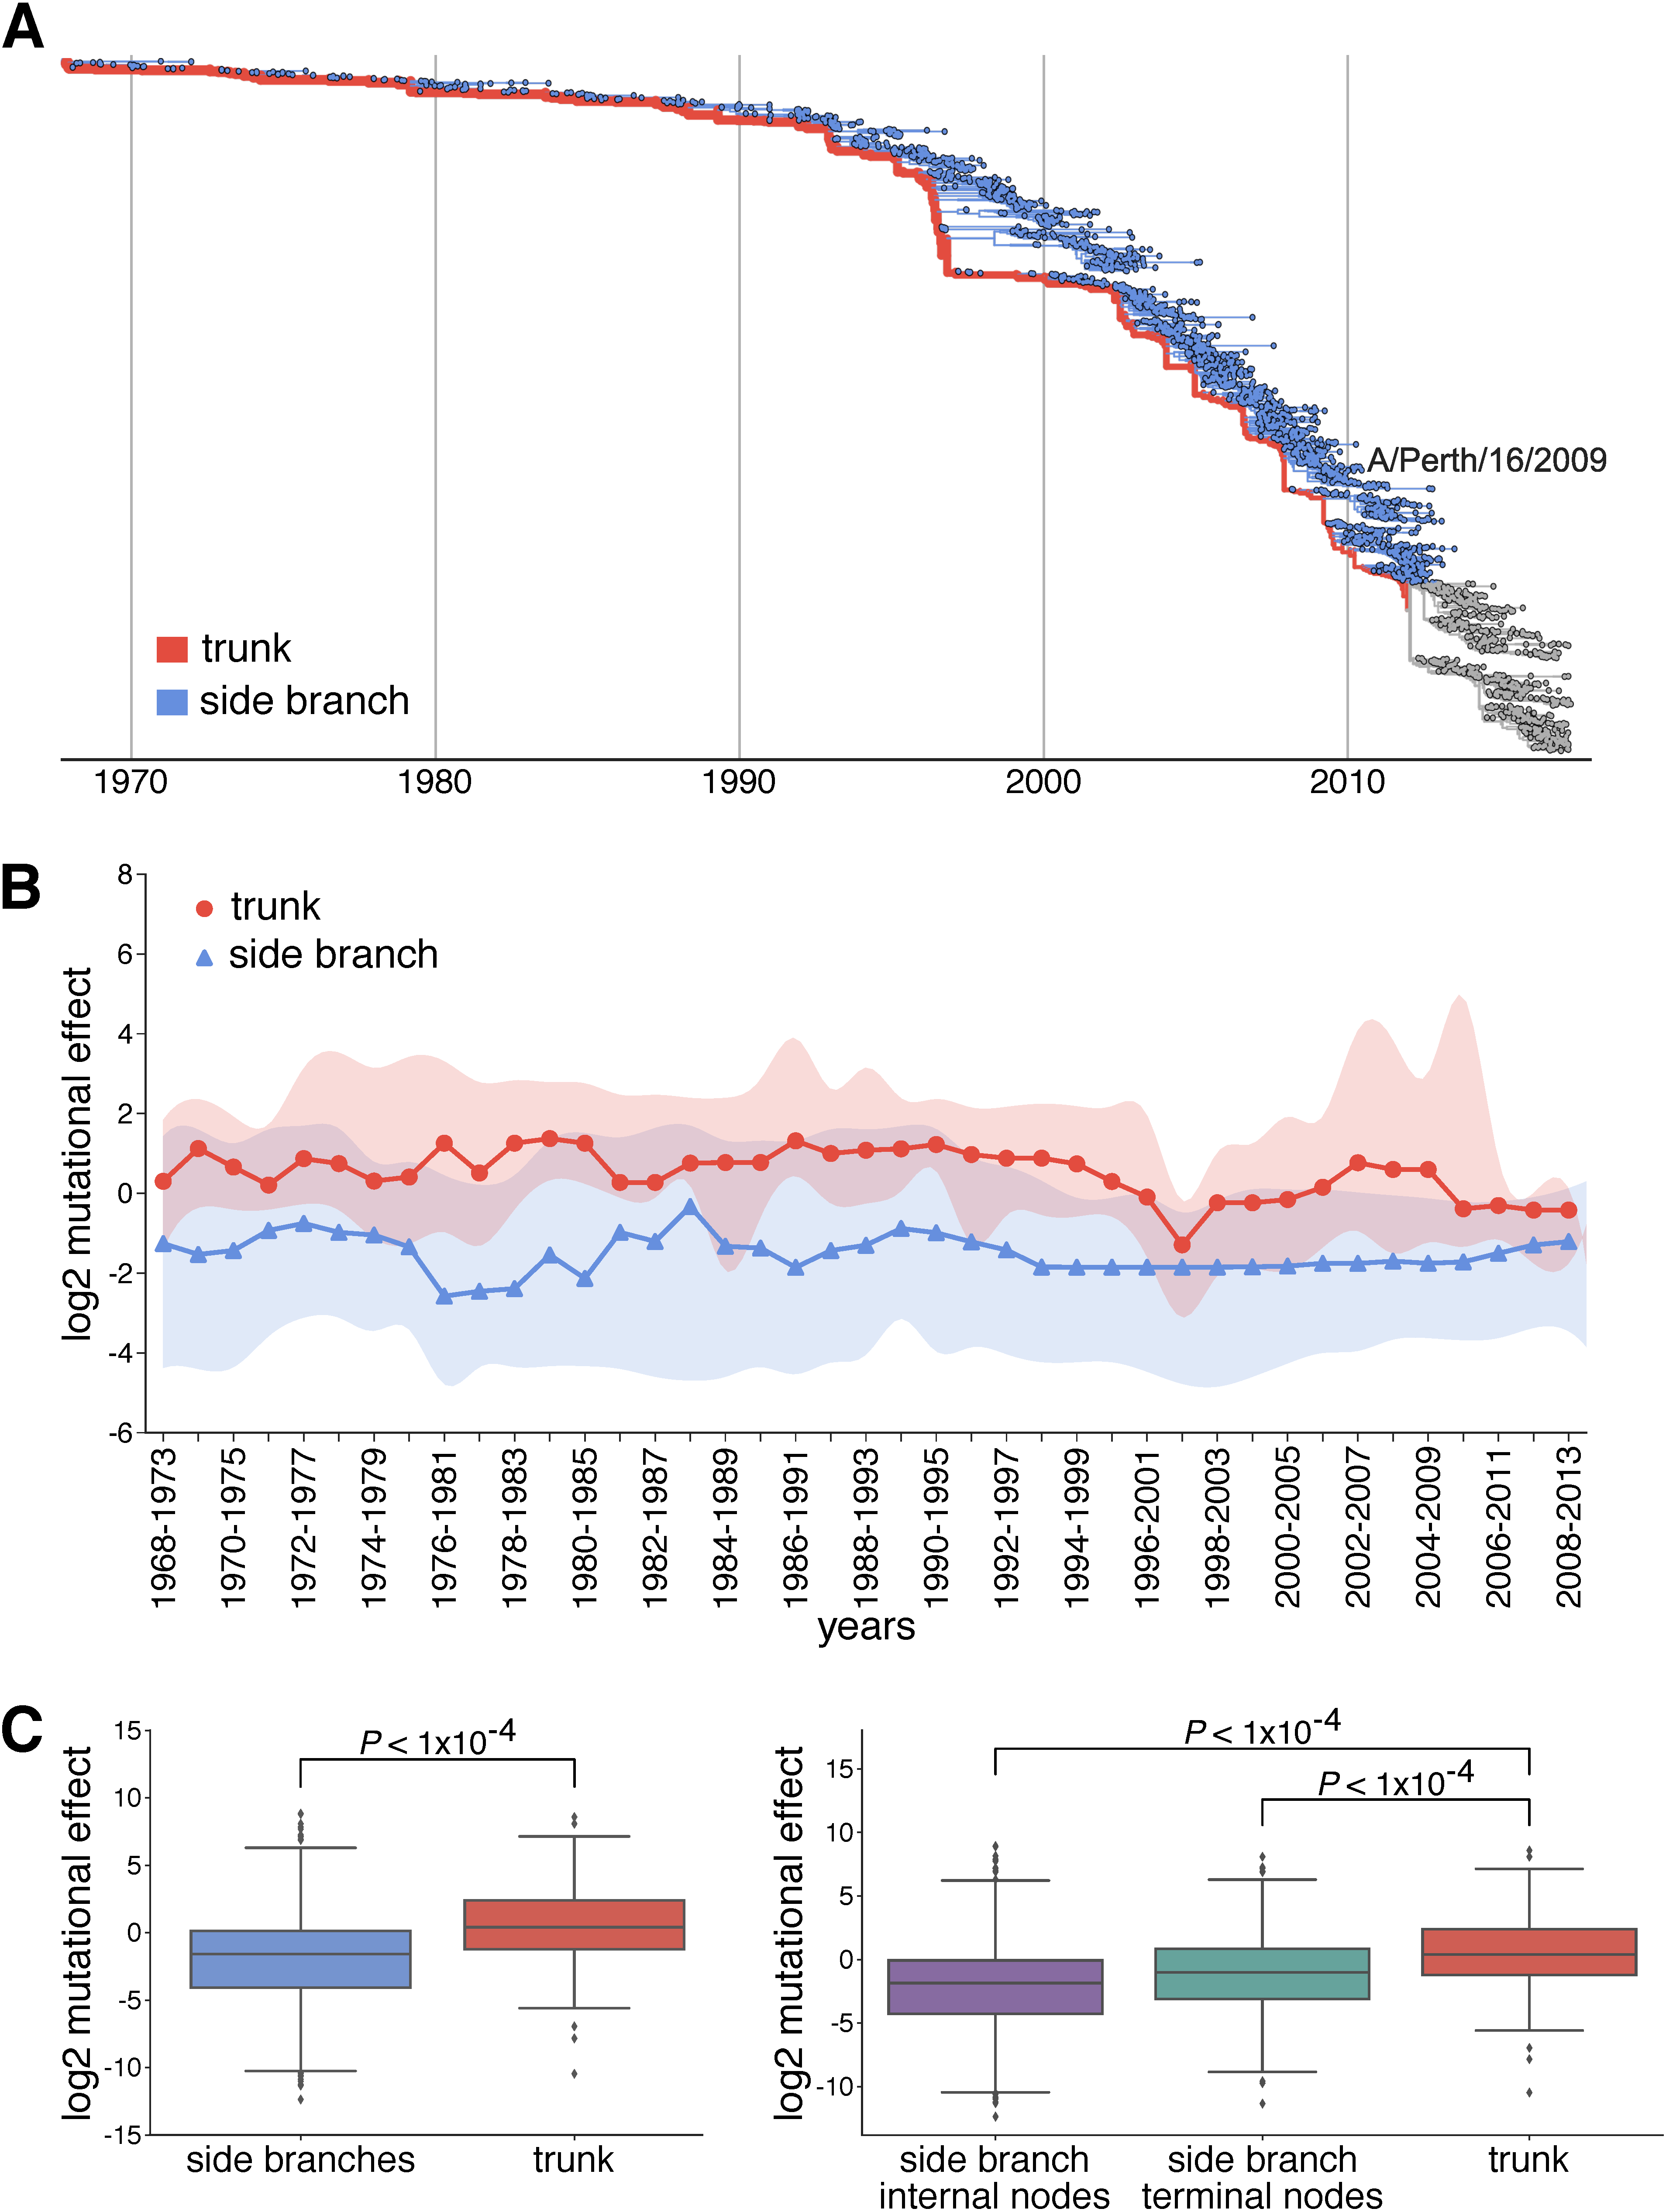
\includegraphics[width=\textwidth]{figs/trunkvssidebranch/trunkvssidebranch.pdf}}
\caption{\label{fig:trunkvssidebranch}
{\bf Mutations in evolutionary successful strains tend to be more favorable than in strains that die out.}
(A) Phylogenetic tree of human H3N2 influenza virus from 1968-present. 
The trunk is shown in red, and side branches are shown in blue.
The gray branches represent the part of the tree for which we cannot yet distinguish the trunk from side branches.
(B) Using the Perth/2009 H3 preferences, we calculated the log$_{2}$ mutational effect for trunk and side branch mutations in windows of 5 years for every year from 1968-2013. 
The median log$_{2}$ mutational effect in a given window is shown as circles for trunk mutations and triangles for side branch mutations. 
The shaded region demarcates the interquartile range of trunk and side branch mutational effects.
The median trunk mutational effects are consistently higher than the median side branch mutational effects for all windows.
(C) The log$_{2}$ mutational effect for all side branch and all trunk mutations (left panel), in addition to all mutations in internal nodes and terminal nodes on the side branches (right panel) are shown.
The preferences were randomized for a number of iterations to estimate significance.
The effects of trunk mutations are higher than side branch, internal and terminal node, mutations.
}
\end{figure}

Rather than estimating an average effect of mutations for trunk and side branch lineages, we can directly compare nodes in the tree by scoring the HA sequence of every node using the preferences to quantify a metric which we will refer to as \textit{sequence preference}.
Figure~\ref{fig:sequence_preference} shows that the sequence preference of trunk nodes tends to be higher than that of side branch nodes.
Interestingly, the sequence preference of all nodes increases over time until it reaches the Perth/2009 node and its closely related nodes, which exhibit higher sequence preference than the trunk. 
The observation that the strain in which we performed our deep mutational scan has one of the highest sequence preferences illustrates epistatic interactions among mutations such that an unpreferred mutation in one background may be preferred in another.
% Due to the sheer number of possible pairwise combinations of mutations, it is impossible for us to experimentally characterize these epistatic interactions among mutations. 
Yet, we are able to distinguish trunk mutations as more favorable than side branch mutations, indicating that the preferences are still of utility over short evolutionary timescales. 

\begin{figure}
\centerline{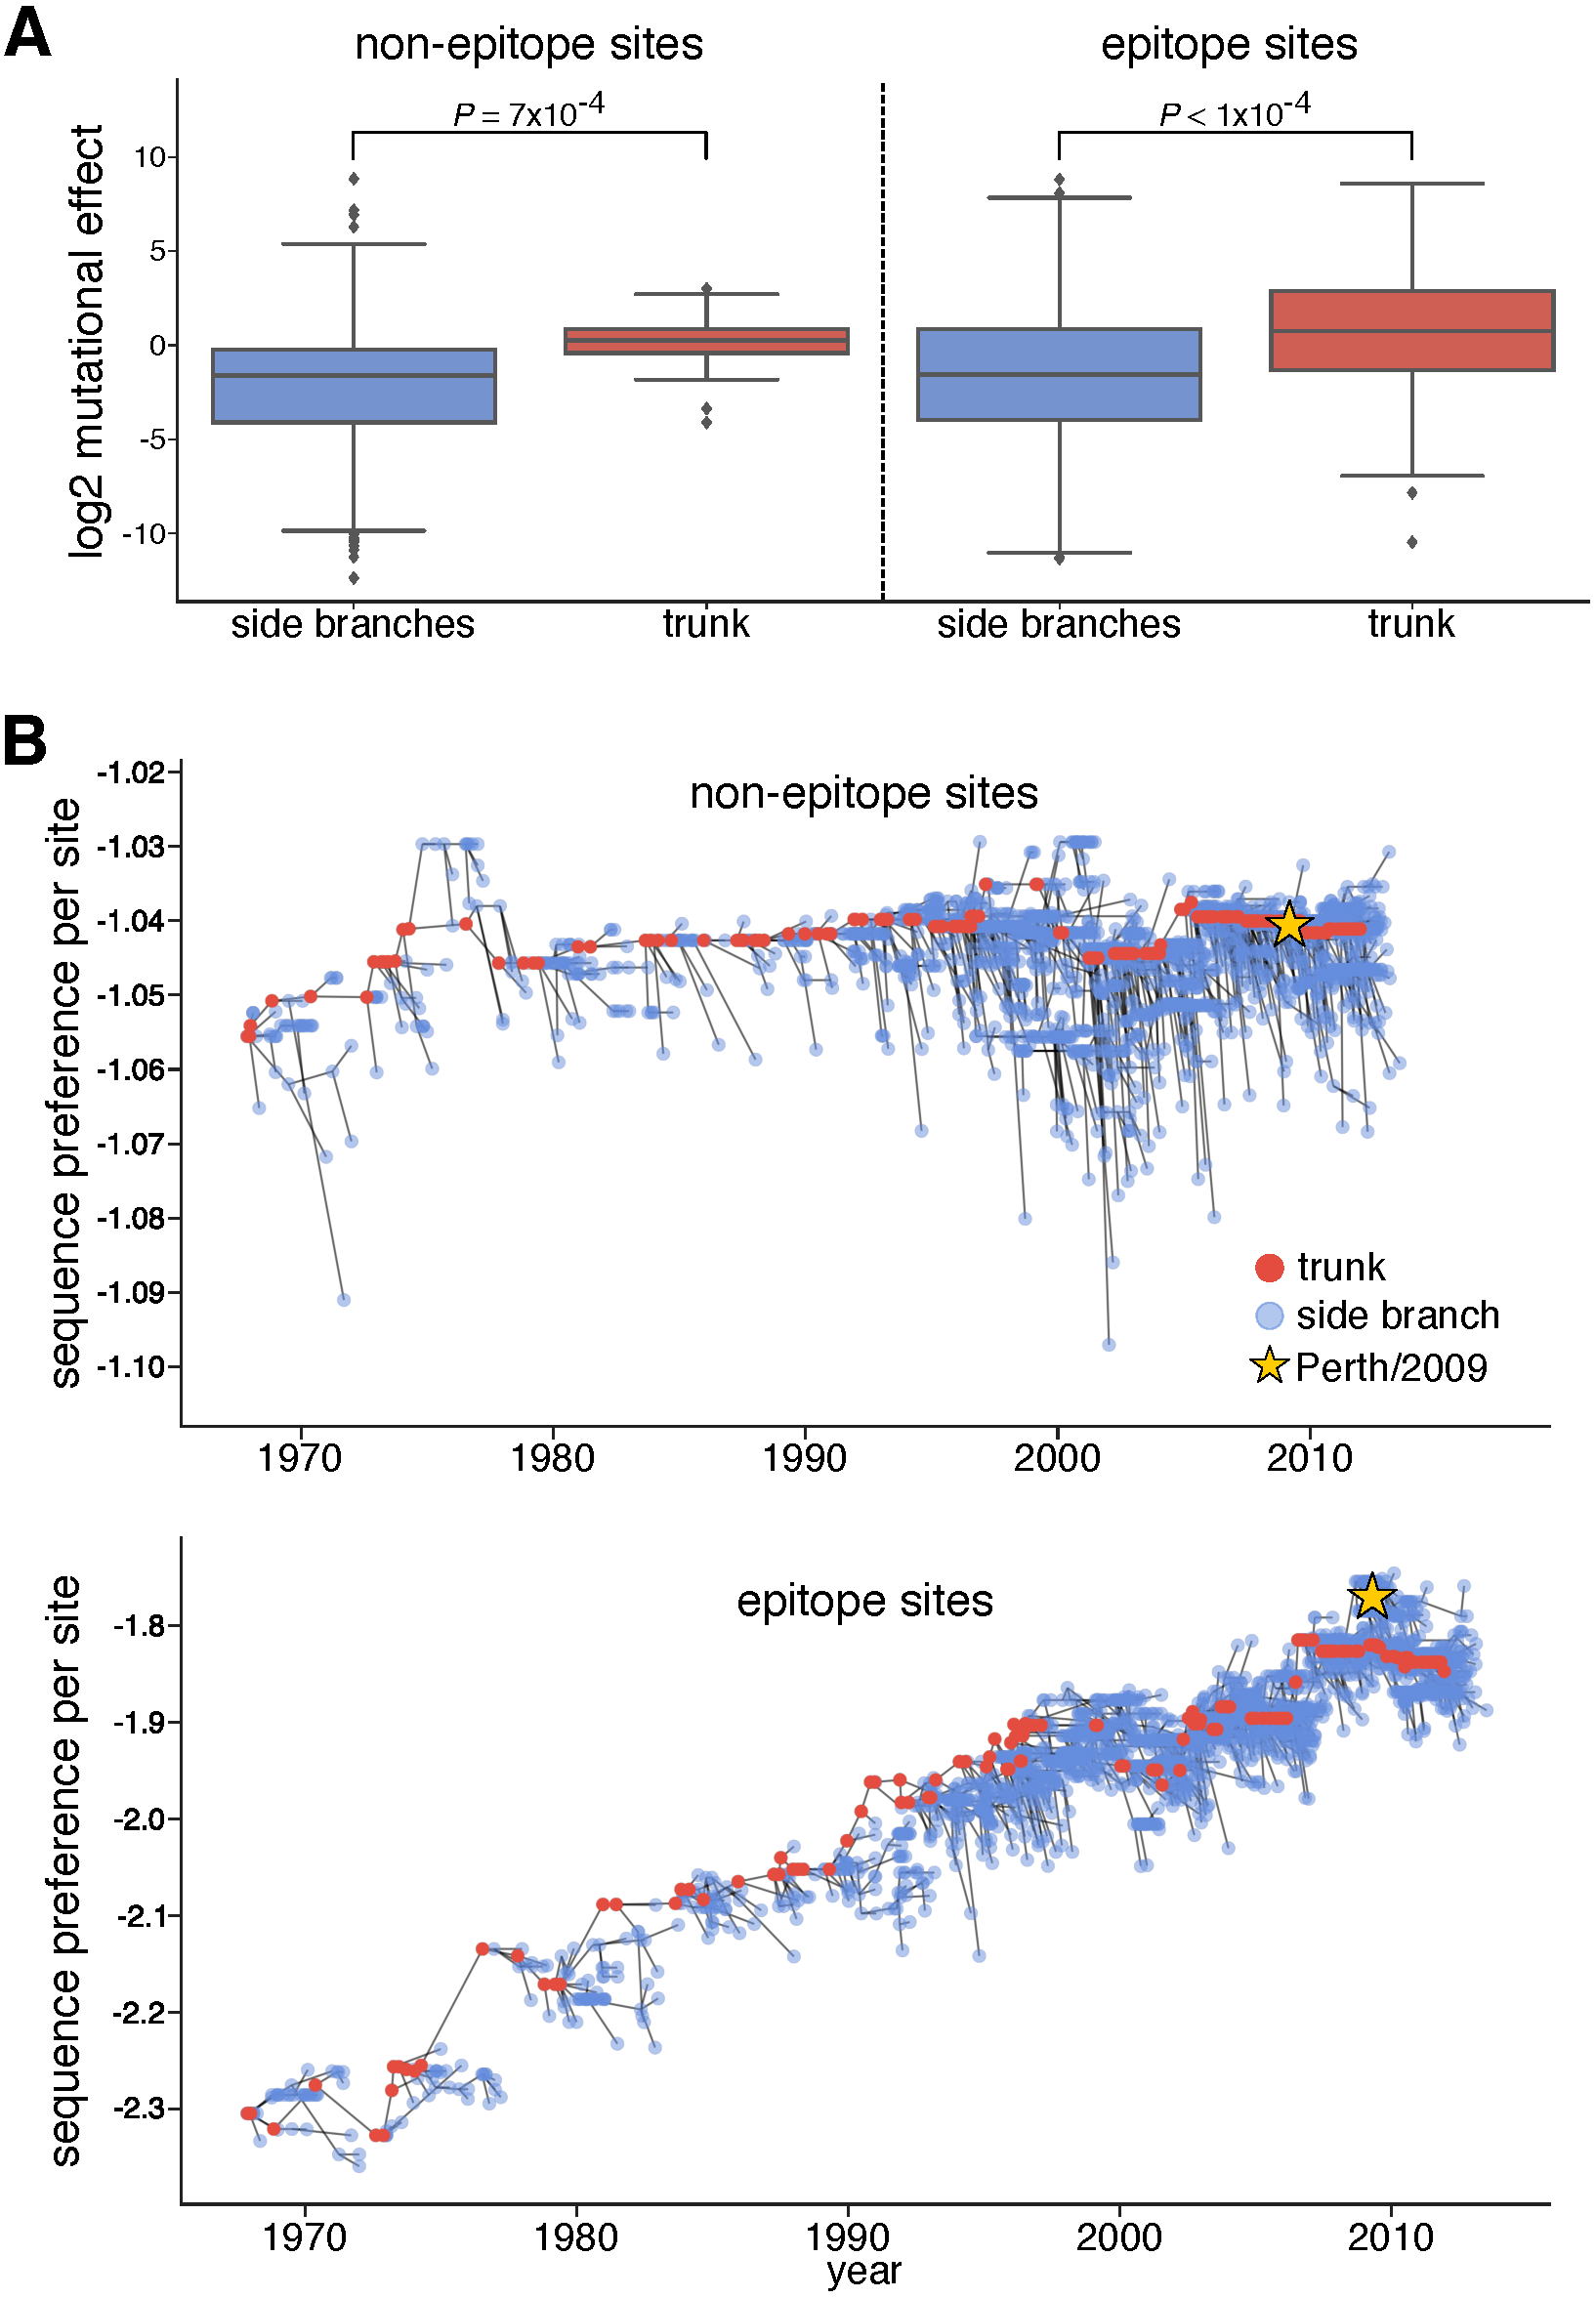
\includegraphics[width=\textwidth]{figs/sequence_preference/sequence_preference.pdf}}
\caption{\label{fig:sequence_preference}
{\bf The trunk exhibits higher sequence preference than side branches.}
figure text
}
\end{figure}

Can we then distinguish lineage-specific mutational effects using the preferences measured in a related HA homolog?
Figure~\ref{fig:WSN_trunkvssidebranch} shows the effect of H3 trunk and side branch mutations as quantified by the WSN/1933 H1 preferences from~\cite{doud2016accurate}.
It is evident that we do not see trunk mutations significantly more favored than side branch mutations using these preferences, suggesting that our ability to discriminate successful and unsuccessful lineages degrades over sufficiently long evolutionary distances. 

\comment{may add text here on using H1 preferences for H1N1 tree}

\begin{figure}
\centerline{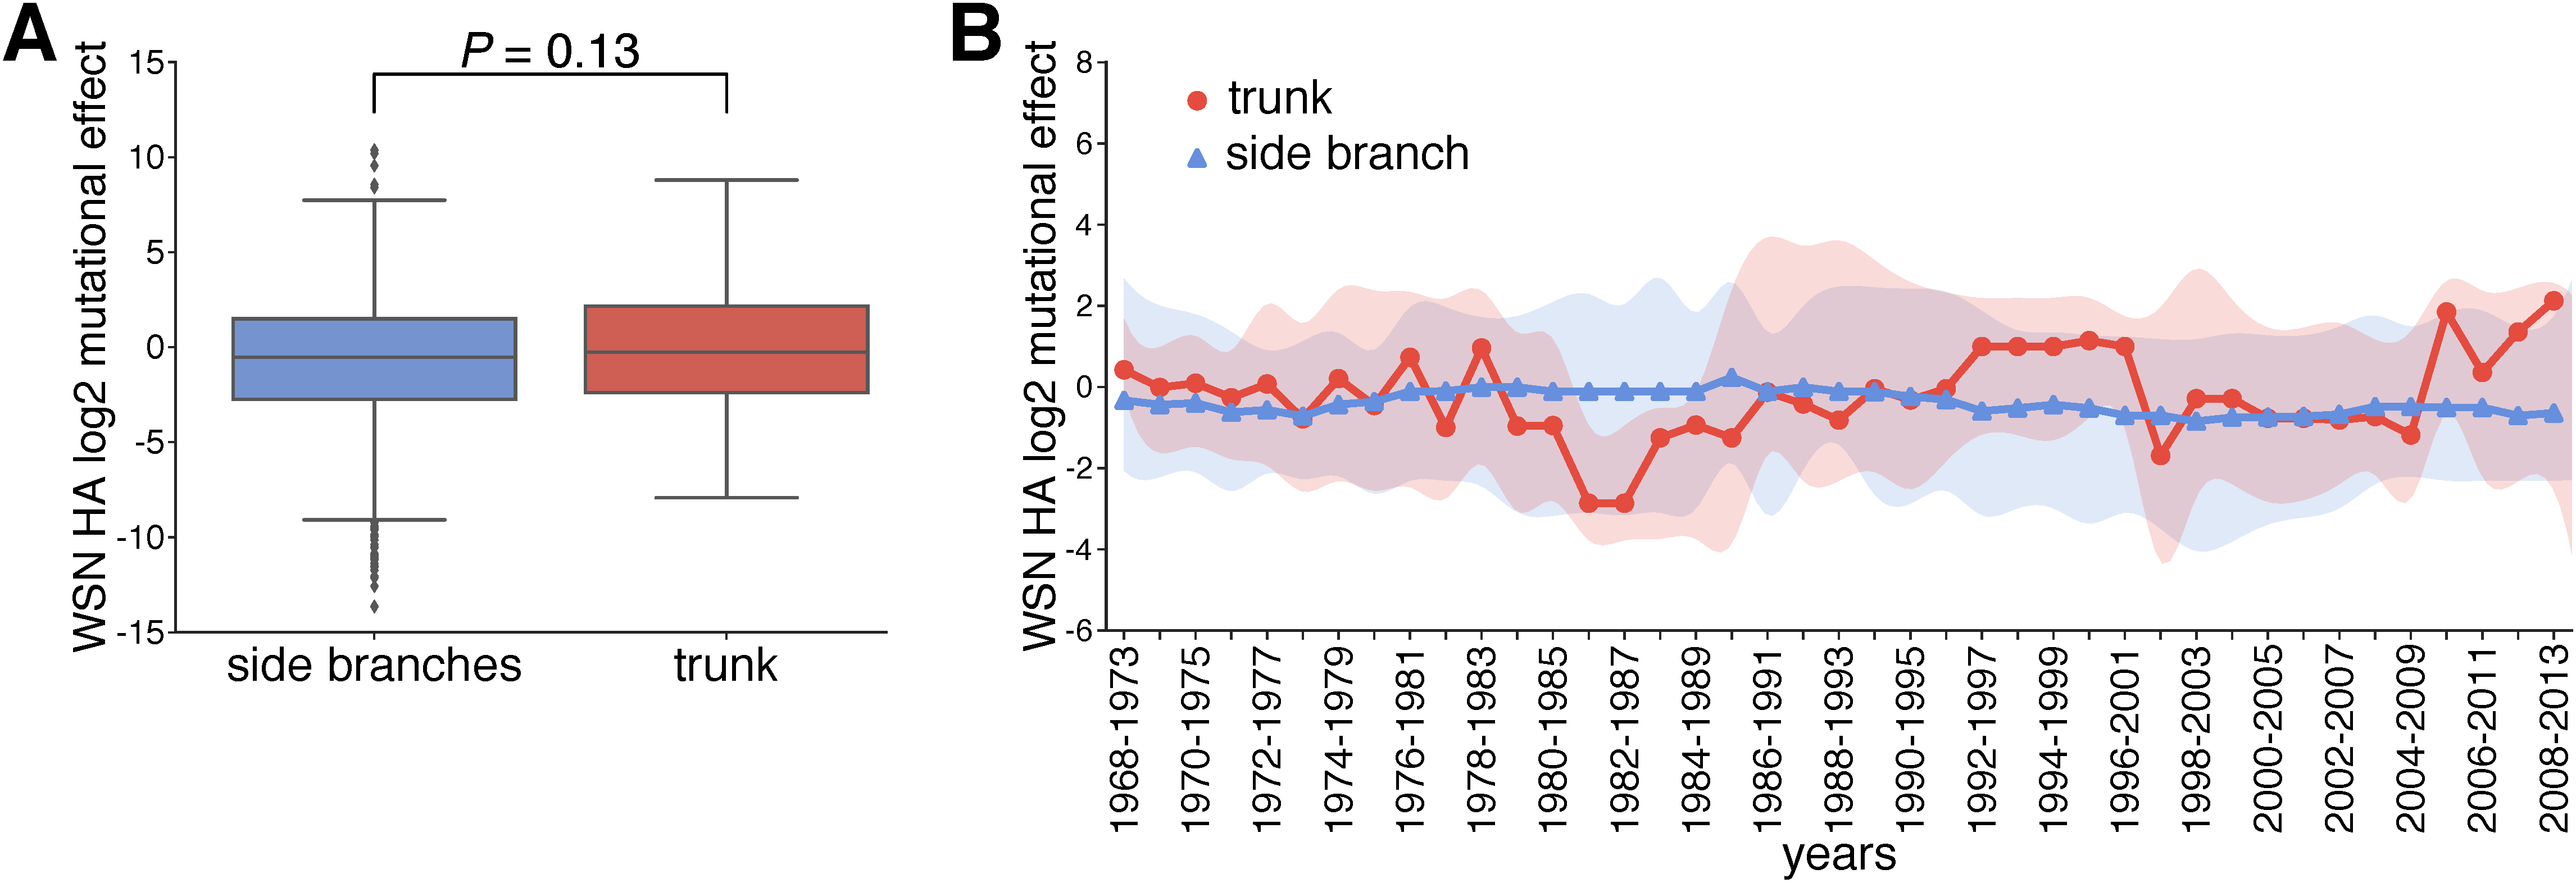
\includegraphics[width=\textwidth]{figs/WSN_trunkvssidebranch/WSN_trunkvssidebranch.pdf}}
\caption{\label{fig:WSN_trunkvssidebranch}
{\bf The WSN/1933 H1 preferences do not reveal differences in trunk vs side branch mutational effects}
(A) We calculated the log$_{2}$ mutational effects of the same set of trunk and side branch mutations from the inferred H3N2 phylogeny in Figure~\ref{fig:trunkvssidebranch} using the WSN/1933 H1 preferences.
There is not a significant difference in trunk vs side branch mutational effects.
(B) We also performed the same sliding window analysis shown in Figure~\ref{fig:trunkvssidebranch}B, but using the WSN/1933 H1 preferences.
There is not a distinct difference in trunk and side branch mutational effects.
}
\end{figure}


\subsection*{Comparing H1 and H3 preferences}

\begin{figure}
\centerline{\includegraphics[width=\textwidth]{figs/distance_distribution/distance_distribution.pdf}}
\caption{\label{fig:distance_distribution}
{\bf The HA homologs exhibit many large shifts in preference compared to shifts for other viral protein homologs}
(A) A phylogenetic tree of the HA subtypes, with the two HA's, WSN/1933 H1 and Perth/2009 H3, for which we have measured amino-acid preferences denoted on the tree. 
The WSN/1933 H1 and the Perth/2009 H3 share $\sim$42\% amino-acid identity.
(B) The correlations of the amino-acid preferences for replicates both within and between the two HA homologs. 
The within-Perth/2009 and the within-WSN/1933 correlations are shown in blue and red, respectively.
The between homolog correlations are in gray.
The correlations for replicates within a homolog are higher than for replicates between homologs.
(C) The distribution of shifts in preference for various homolog pairs are shown.
}
\end{figure}

\begin{figure}
\centerline{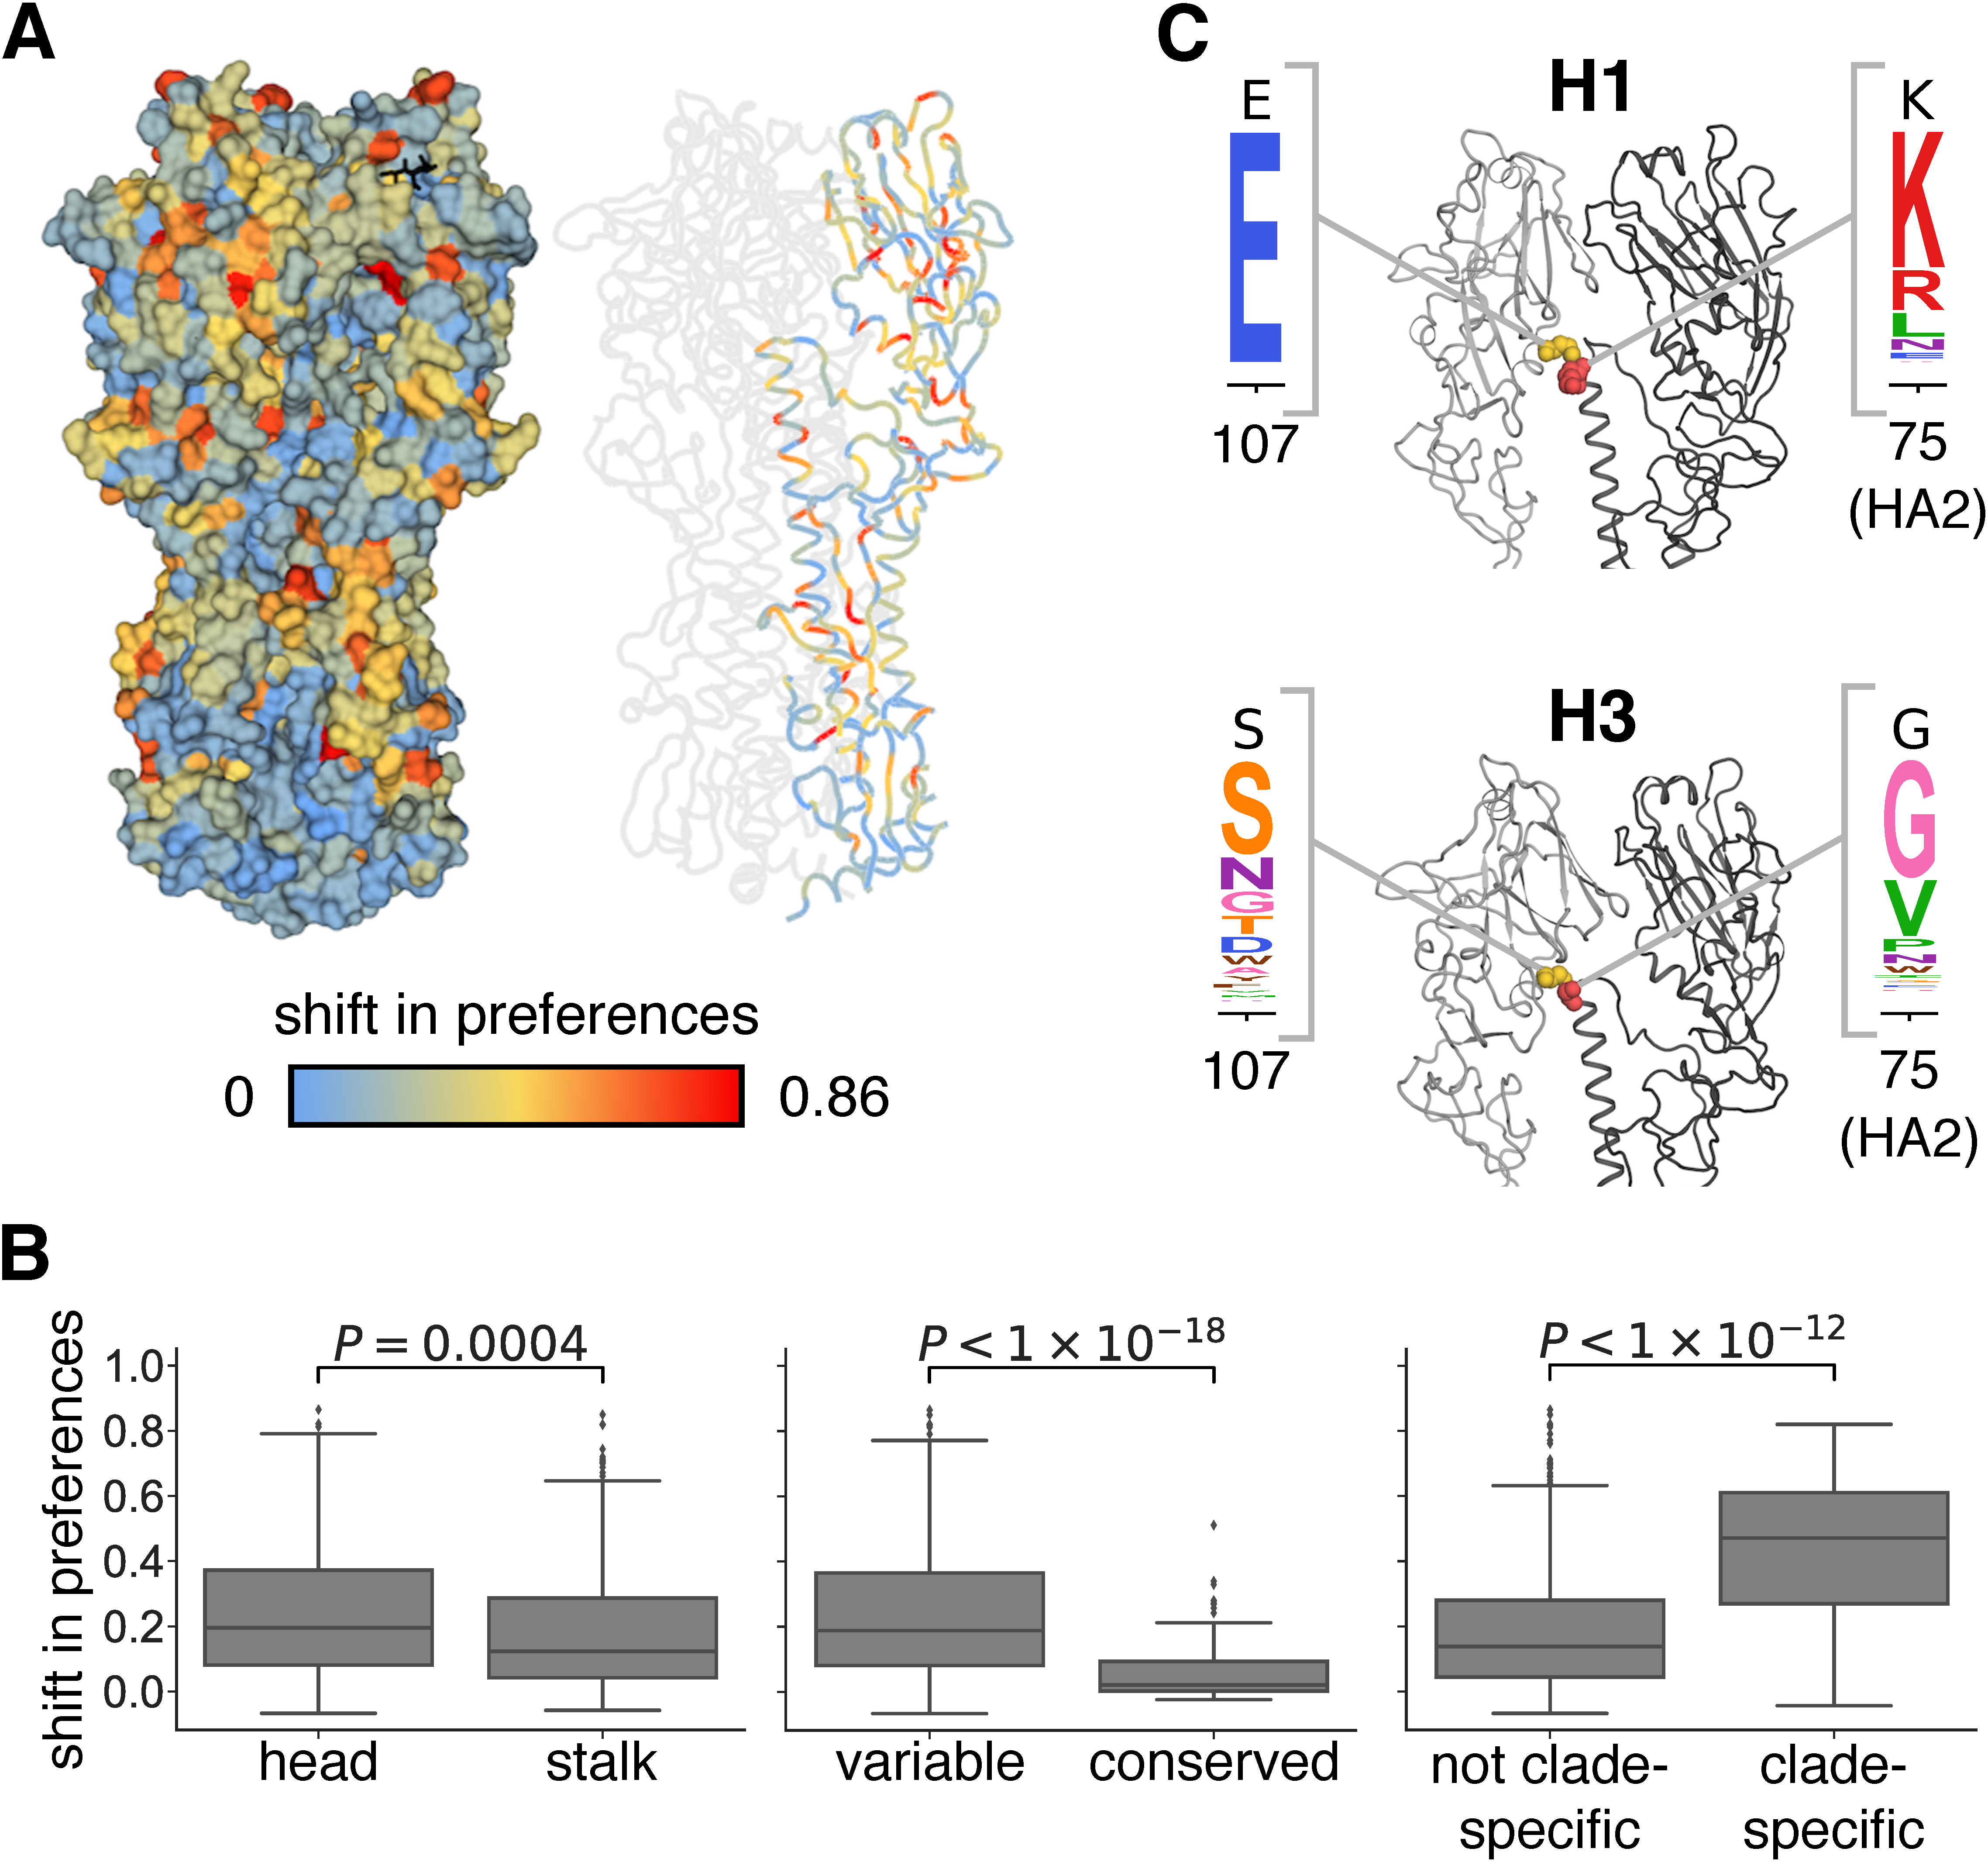
\includegraphics[width=\textwidth]{figs/RMSD_heatmap/RMSD_heatmap.pdf}}
\caption{\label{fig:RMSD_heatmap}
{\bf Shifts in preferences mapped onto the structure of HA}
(A) The preference shifts as calculated by $RMSD_{corrected}$ between the two HA homologs is mapped onto the structure of HA (PDB 4O5N, citation). 
The left structure shows the HA trimer, and the right structure colors one of the monomers. 
The sialic acid receptor is shown in black sticks.
Gray indicates little shifts in preference, while red indicates large shifts in preference.
The top ten most shifted sites are shown in spheres on the monomer.
(B)
}
\end{figure}


\section*{DISCUSSION}


\clearpage
\small

\section*{METHODS}
\label{sec:methods}
\subsection*{HA numbering}
Unless otherwise indicated, all sites are in H3 numbering, with the signal peptide in negative numbers, the HA1 subunit in plain numbers, and the HA2 subunit denoted with "(HA2)". The conversion between sequential numbering of the A/Perth/16/2009 HA and H3 numbering was performed using an HA numbering Python script (available at \url{https://github.com/jbloomlab/HA_numbering}).

\subsection*{Creation of MDCK-SIAT1-TMPRSS2 cell line}
The human TMPRSS2 cDNA ORF was ordered from OriGene (NM\_005656), PCR amplified, and cloned into a pHAGE2 lentiviral vector under an EF1$\alpha$-Int promoter and attached to mCherry through an IRES...etc etc
\comment{Need to look at Katie's notebooks for this...}

\subsection*{Generation of HA codon mutant plasmid libraries}
Recombinant A/Perth/16/2009 (HA, NA) $\times$ A/Puerto Rico/8/1934 influenza virus, NIB-64, NR-41803 was ordered from BEI Resources, NIAID, NIH. 
Bulk RNA from the viral sample was extracted using the QIAamp Viral RNA Mini Kit (QIAGEN) according to manufacturer's instructions.
The Perth/2009 HA and NA genes were then reverse transcribed, PCR amplified, and cloned into the pHW2000~\citep{hoffmann2000dna} and pICR2 \comment{cite?} plasmid backbones.

The codon-mutant libraries were generated using a PCR-based approach described in~\cite{dingens2017comprehensive}.

\subsection*{Generation and passaging of mutant viruses}
The mutant virus libraries were generated and passaged using the approach described in~\cite{doud2016accurate} with several modifications.

\subsection*{Barcoded subamplicon sequencing}


\subsection*{Analysis of deep sequencing data}

\subsection*{Inference of phylogenetic trees}
\comment{We downloaded X sequences from the Influenza Virus Resource ?.... etc. inferred the tree, ancestral state reconstruction, visualized the tree. Mark Perth/2009 on the tree}
To parse out trunk mutations from side branch mutations, we first defined a set of recent nodes sampled on or after Jan. 1, 2017, and traced these nodes back to their most recent common ancestor. 

\subsection*{Quantification of mutational effects and sequence preferences from an H3N2 phylogeny}

\subsection*{Data availability and source code}
Deep sequencing data are available from the Sequence Read Archive under BioSample accessions SAMN08102609 and SAMN08102610. Computer code used to analyze the data and produce the results in the paper are in...


\subsection*{ACKNOWLEDGMENTS}
We thank Sarah Hilton, Hugh Haddox, Sidney Bell...the Fred Hutch Genomics Core...
Funding...


\bibliographystyle{mbe}
\bibliography{references.bib}

\clearpage
\normalsize

\end{document}